\pagestyle{plain}

\subsection{Results evaluation}

Main result of this project is Python code for automatical analysis of TEM images of gold nanoparticles and nanorods. This code was debugged using input image \ref{fig:20nm}, because it is the most ideal image, there are advantages of this image: pretty good resolution, number of particles, fairly good contrast and homogeneous background. This image has also imperfections which can be used for solve these frequent issues, which are overlapping particles, hight resolution of image and small bright spots on particles. Overlapping particles were solved by using combination of two segmentation methods. Watershed transform was used for find all particles, but watershed divides ovelapping particles in the middle so it decreases its area, in some cases it even cannot divide some particles. So hough transform which finds specific shapes in image is used for detecting circles, this method is used just for areas with ovelapping particles. High resolution issue and bright spots are descibed in chapter \ref{image_errors}. Result of this sample image can be seen on figure \ref{fig:res20nm} and histogram of sizes of this image can be seen on figure \ref{fig:hist20nm} in chapter Results.

\subsection{Sample preparation errors}\label{measurment_errors}

The goals of the project were to prepare TEM samples on copper gird and acquire TEM images. Samples of nanoparticles and nanorods were prepared, but during TEM measurment there were another small particles on some samples. Theese small particles were DNA fragments and it means that some of grids must be used before and returned into box with new grids. This accident may cause errors during image segmentation while theese small particles are not removed well. This false detection of DNA particles can be seen on figure \ref{fig:res50nm}.

\begin{figure}[h!]
\begin{center}
    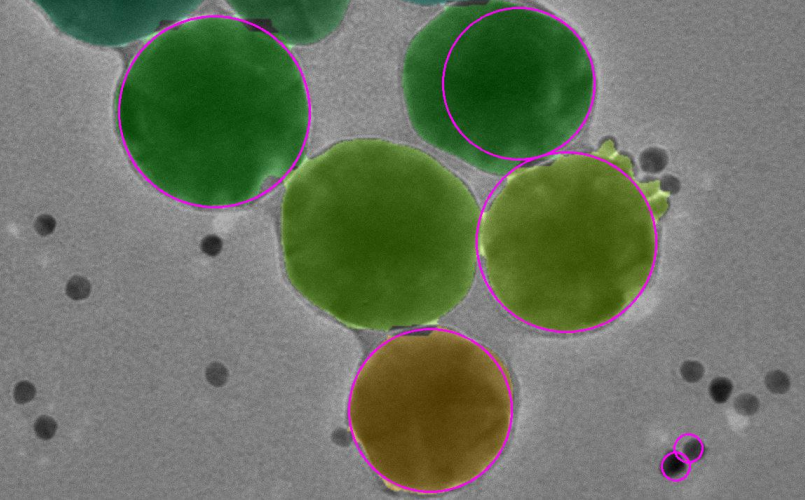
\includegraphics[width=0.5\linewidth]{res80nm.png}
    \caption{False detection of DNA particles in 80 nm nanoparticles TEM image}~\label{fig:res50nm}
\end{center}
\end{figure}

Another source of segmentation errors may be insufficiently dried samples. Samples of nanorods with absorption peak 800 nm can be seen on image \ref{fig:NRs}, this iimage has inhomogeneous background due to it was measured while sample was still a little wet. This is error which may happen more frequently so it is treated in software, however it declines quality of image. Wet sample can be seen on figure \ref{fig:wet}.

\begin{figure}[h!]
\begin{center}
    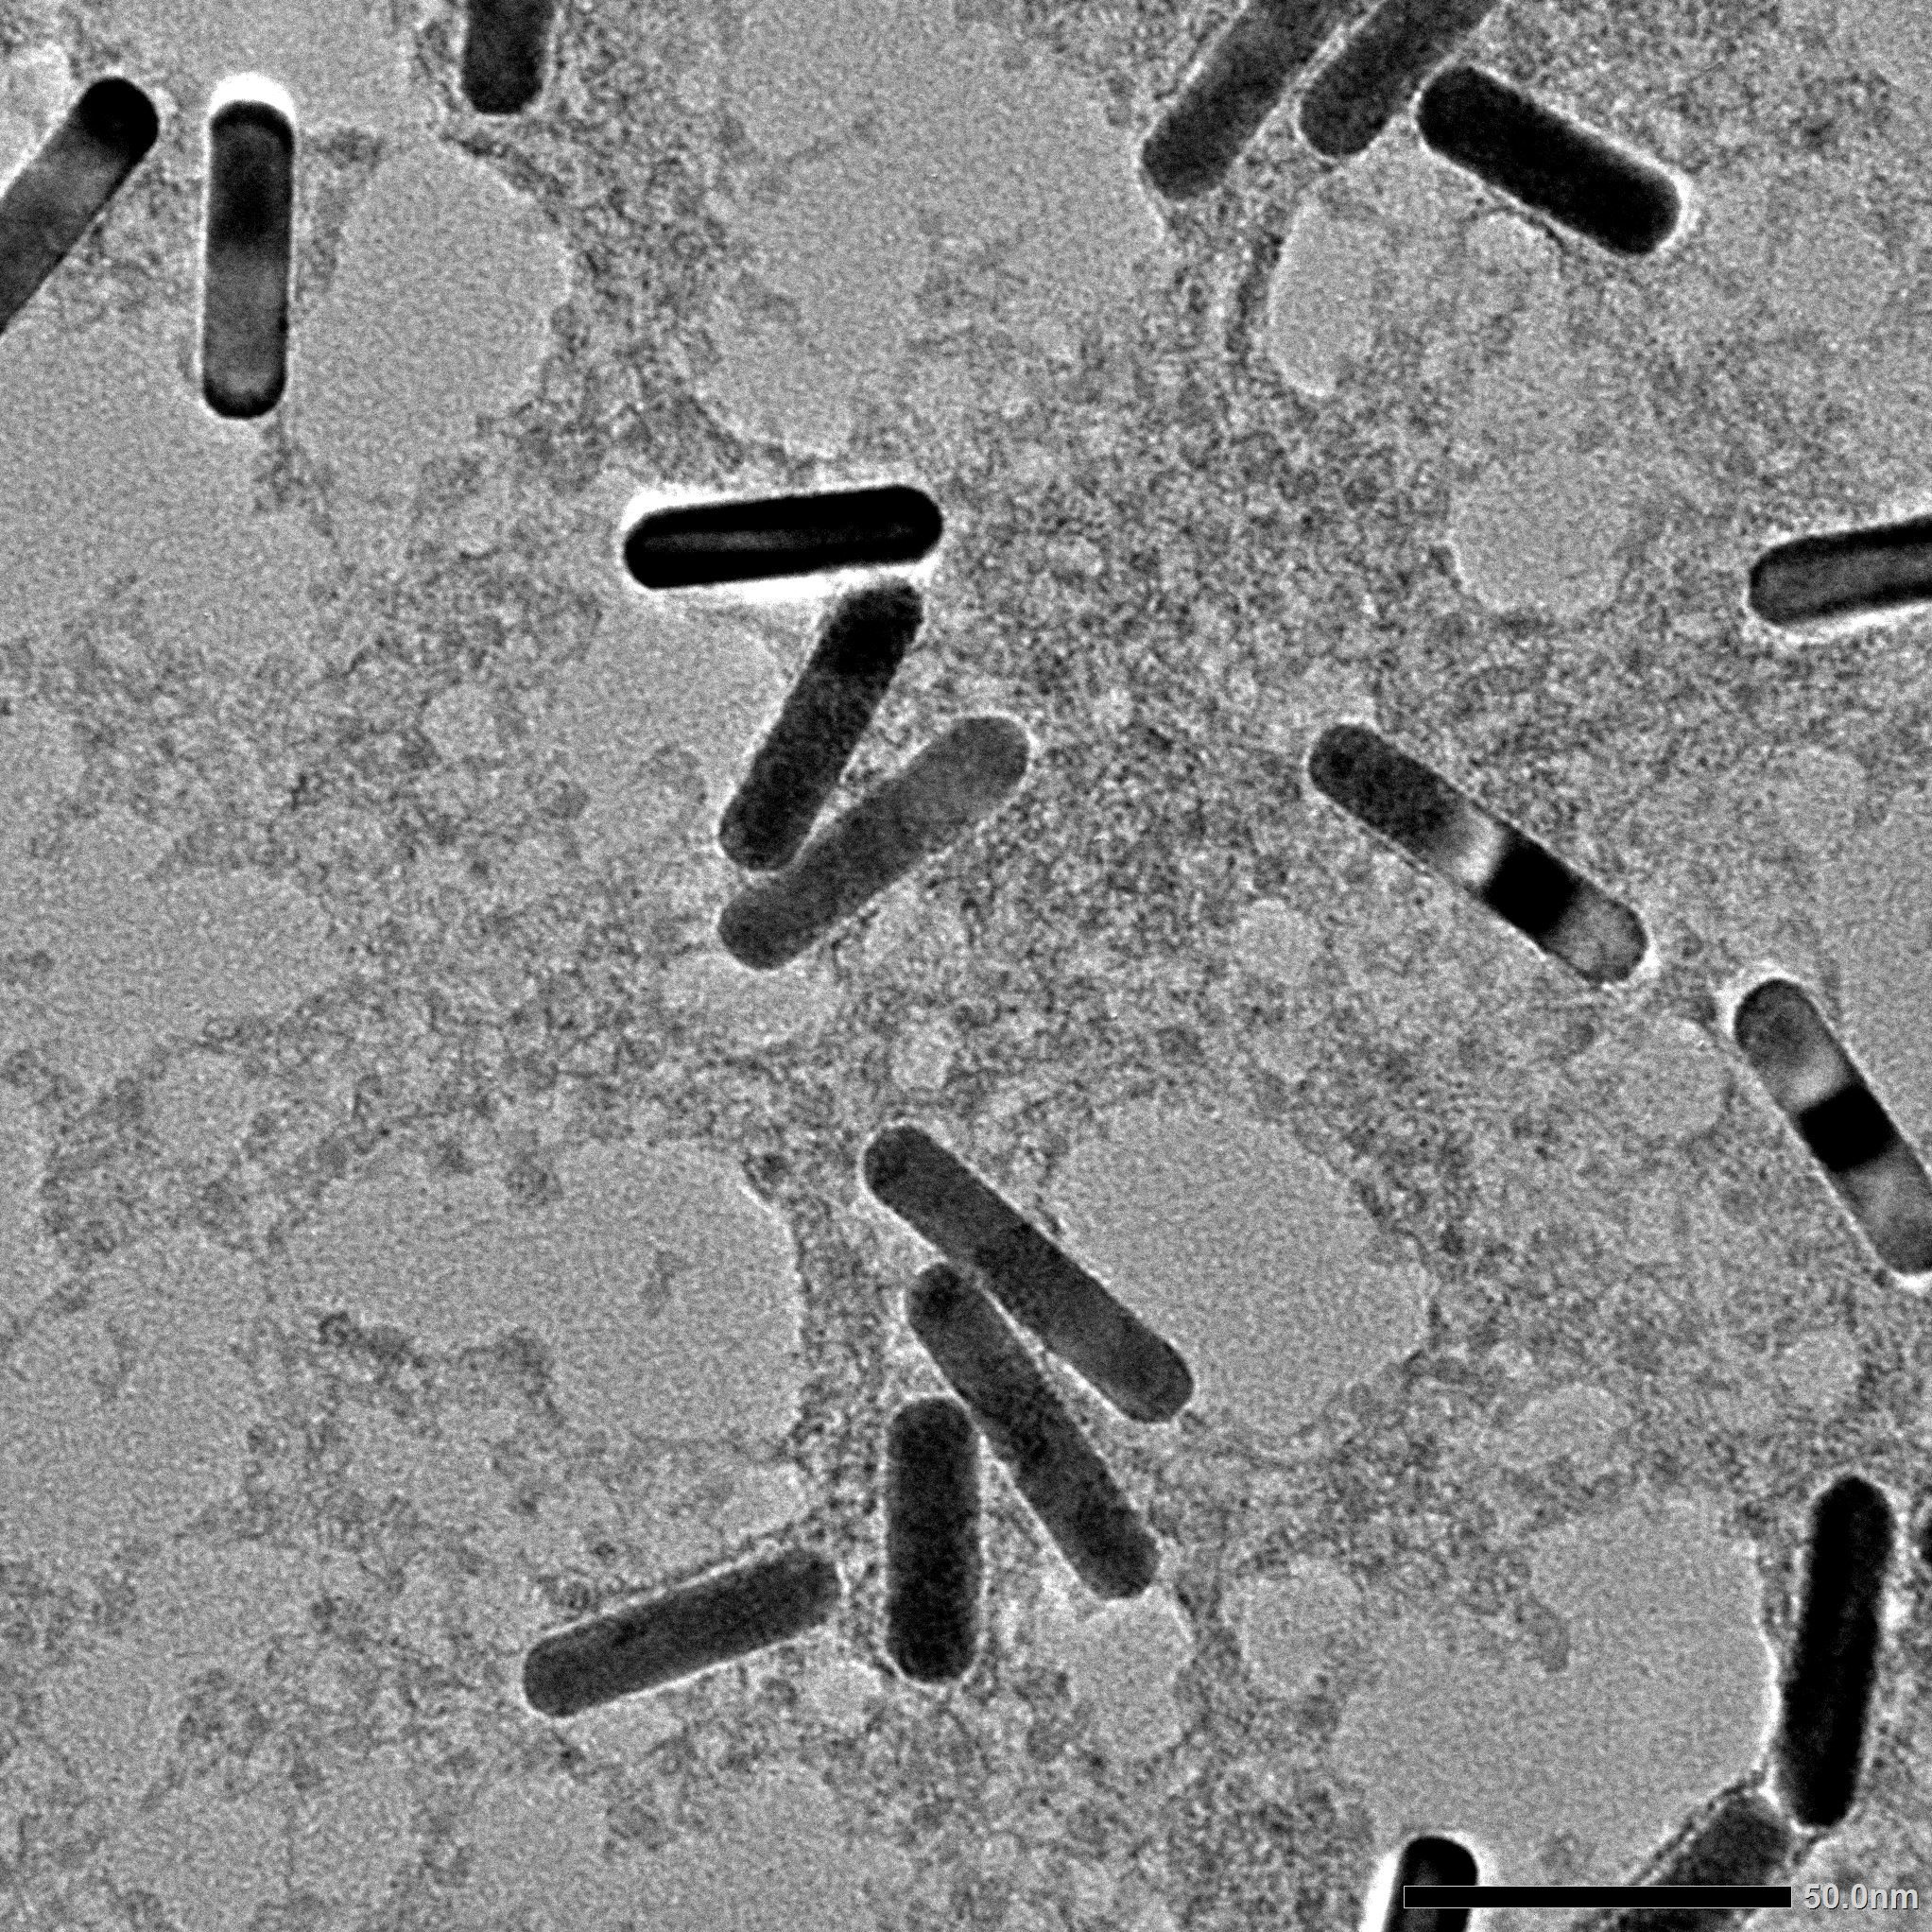
\includegraphics[width=0.5\linewidth]{wet.jpg}
    \caption{Inhomomogeneous background caused by wet sample}~\label{fig:wet}
\end{center}
\end{figure}

\subsection{TEM measurment errors}\label{image_errors}

Another sources of potential errors can by quality of TEM images. There are several issues which affects results of image analysis program. First issue is resolution. Microscope computer saves images in very high resolution 2044 x 2044 pixels and due to computational complexity of most functions, image resolution has to be reduced. For most of images rescaling does not matter, but there are images where particles are very tiny in compare with image size (example of this case can be seen on figure \ref{fig:40nm} (b) or figure \ref{fig:NRs} (b) in chapter Results). After rescaling theese particles have diameter for example 8 or 9 pixels, so accuracy of measurement extremely decrases. Solution for this problem could be manually cropping thees images before automatical analysis, but there is an issue. Images contain scale bar and it is located in corner of image and it is used to determine pixel size, so cropping image would remove this information. Appropriate solution for this problem was not found and it will be part of following project.

Another issue with TEM images quality can be contrast. Algorithm for particles analysis works on principle of substracting particles from background based on pixel intensity. Particles in some images contain stains with higher intensity which is similar or even higher than background intensity. So algorithm assigns these pixel to background not to particles. This issue is partly treated in code by using morfological operation for filling holes. This solution can solve smaller bright spots but it cannot do anything with cases where for example half of particle is bright. Some TEM images have low contrast overall so thresholding methods may not be so accurate it could be. Example of low contrast nanorods with even bright spots can be seen on \ref{fig:resNRs} (a) in chapter Results. In this image wet background is also problem, so it decreases quality of image even more. Bigger bright spots may cause oversegmentation of image. This case can be seen on figure \ref{fig:oversegment}.

\begin{figure}[h!]
\begin{center}
    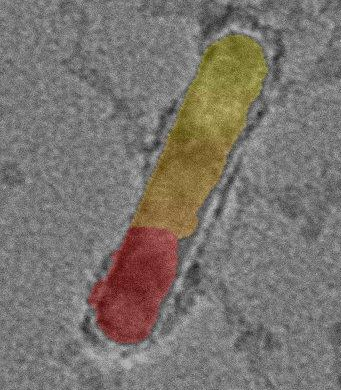
\includegraphics[width=0.5\linewidth]{oversegment.png}
    \caption{Oversegmented nanorod}~\label{fig:oversegment}
\end{center}
\end{figure}

Last issue which is related to image quality and occured in sample images is badly focused image. It is problem especially in images with large number of small particles, because particles in samples are overlapping and in this case it is almost impossible to divide them well. Example of this case can be seen on figure \ref{fig:bad_focus}.

\begin{figure}[h!]
\begin{center}
    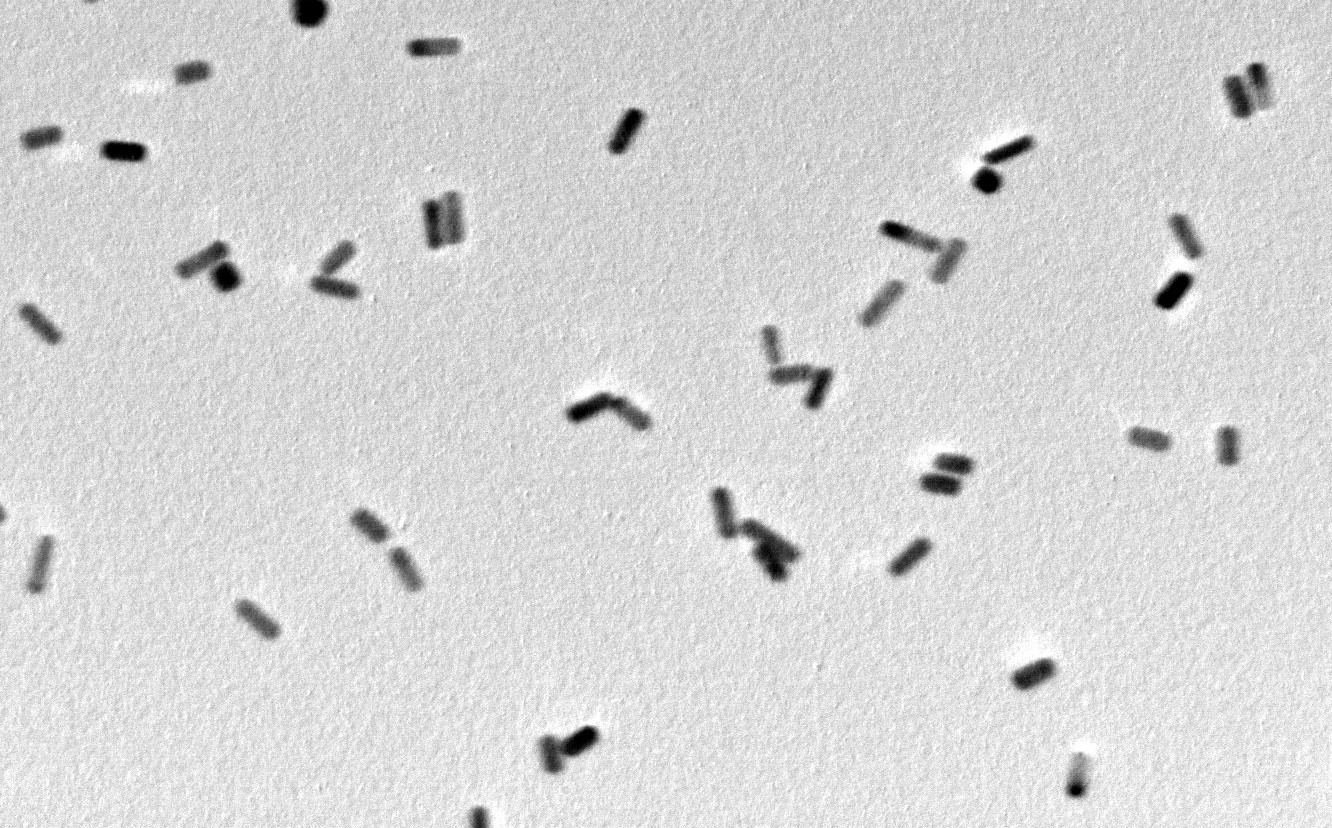
\includegraphics[width=0.5\linewidth]{discNRs.jpg}
    \caption{Bad focused nanorods}~\label{fig:bad_focus}
\end{center}
\end{figure}

In speech about overlapping particles there is also one issue with this which cannot be solved. Some samples contain places with a lot of particles laying on each other. In some extreme cases there is not even possible to see individual particles. This images obviously cannot be used for analysis. Program detects these huge clusters as one particle and it would bring enormous error in results so program have treated these cases removing such huge areas which were detected as one particle. Example of image with this case can be seen on figure \ref{fig:big_spot}.

\begin{figure}[h!]
\begin{center}
    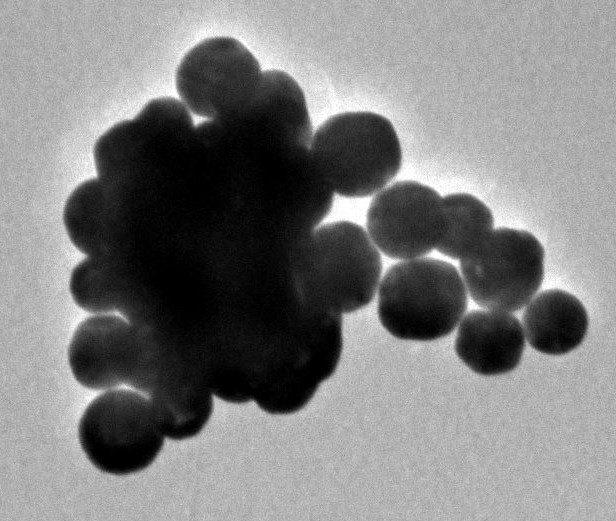
\includegraphics[width=0.5\linewidth]{disc80nm.jpg}
    \caption{Image with huge cluster of particles}~\label{fig:big_spot}
\end{center}
\end{figure}

Last issue which was recorded is fact that microscope computer saves data into jpg format. It is understandable because jpg in compare with tiff has far lesser size, but compresses data and by compressing artifacts may occur. This can be problem in cases where original image have region with zero pixels and compressing causes that pixels with higher value (1, 2, 3 etc.) occur in this region, example of this region is scale bar. In image analysis program scale bar is detected by intensity threshold and artifacts may cause errors in this detection. It was solved by detecting more than just zero pixels and than taking just the biggest reion which is obviously scale bar.

\subsection{Calculations}

The main goals of this project is to create program which can automatically calculate sizes of nanoparticles and shapes of nanorods. Program returns histogram of diameters for nanoparticles and histogram of major and minor axis length for nanorods and also txt file with sizes of all particles, average sizes and for nanorods also aspect ratio. Errors in this section may be cause by all the cases described in chapter \ref{measurment_errors} and \ref{image_errors}. Detecting wrong particles may cause wrong average size, so particles which are too small or too big are removed. Some false particles may still not be removed due to many reasons so it may cause errors in results. Another source of results errors may be in resolution issue. If there is only a few pixels in one particle, accuracy of measurement extremely decreases. On figure \ref{fig:hist2} is example, where number of pixels in one particle was so small, that difference between particles were just in one pixel. This particles have diameter 8 and 9 pixels and when pixels are transformed into size in nanometers, it created this histogram.

\begin{figure}[h!]
\begin{center}
    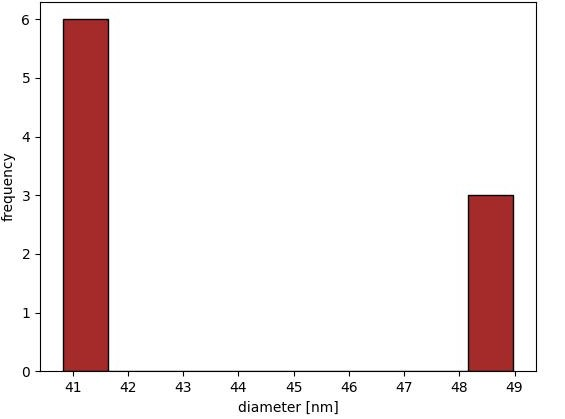
\includegraphics[width=0.8\linewidth]{hist50nm.jpg}
    \caption{Histogram with just two sizes}~\label{fig:hist2}
\end{center}
\end{figure}